\section{Introduction}
This chapter will discuss all of the design choices that were made during the production of the fitness monitoring web application Recur. It will go into more detail about the grid behind the design, why responsive web design is important, and will talk about the design of the database used to store all the application's information. \\

\section{Grid design}
\citet{bertoni:2002} states that the concept of minimalist architecture is to strip everything down to its essential quality to achieve simplicity. The design of the application was to follow this simple rule. The bare essentials were the only aspects that needed to be displayed to the user. The set up of the website is to have three blocks displayed in the centre of the screen, laid out on a six column grid. Grid design is important in web design as it adds continuity to each page. Each page will have the relevant information in a similar position to the last, allowing the user to be able to extract the information more quickly. A grid layout also makes it easier to design for other devices. \citet{walkers:2013} found that their mobile traffic was up to 29\% in Q2 2013. From this, we can see that more and more people are browsing the internet from the mobile devices. 43\% of this traffic was from iPhones. One of the key challenges facing web designers is to make sure that our web applications look as good on a 320 pixel width devices as it does on a laptop monitor. This leads to the design of the application being based on a six column grid. This was for two main reasons: the first being to keep consistency through the sizing of different areas of the website and the second being it makes it much easier to scale the design down for mobile traffic. Due to the fact that mobile traffic is increasing, and also that the application will mainly be used on mobiles, responsiveness was very important when designing the application. It need to have the same feel on a 1920px screen as it would on a 320px mobile device screen.\\

\section{Wireframe and mock up}
Simple designs were sketched up in a notebook to get a feel for how each of the pages would look on both a normal monitor and a mobile devices. After sketches were complete, they were then drawn up in Sketch \citep{sketch:2013} where colour, text, and images can be added to get an even better feel for how the application is going to look and work. Once colour could be applied to the design, user accessibility could be thought about. Around 8\% of men in the United Kingdom are affected by some form of colour blindness and 0.5\% of women \citep{colourBlind}. If the design was to ignore their needs then there would be a percentage of the population that would be unable to use the application. For this reason, colour should never be the primary cue for information. During the design process, changes were made so that any occurrence where colour was the primary cue would also have a visual cue. For example: when the user checks off a goal, the text will have a strike through it as well as turning red. Also, a large percentage of the population have a visual impairment. A few steps were taken to keep the site safe for the visually impaired. The font size and weight is kept at a easy to read level so that it is not taking up to much space but is still easily readable. Also, the colour of the font has to contrast with that of its background. From a previous design, the background of the cards and headers was very light and the font colour was too light which would be quite difficult to read for a visually impaired person. Since then, the background colour has completely changed to a darker blue and the colour of the text has been made a lighter shade of grey. As for the typeface, Helvetica was chosen, as san-serif fonts are easier to read for the visually impaired. Where there is any large amount of text that the user will need to read, a line height of 1.5 will be used to make it easier to read for visually impaired people. Also, using ARIA HTML5 \nomenclature{HTML}{HyperText Markup Language} landmarks, such as header, footer and nav tags, will increase the usability of my website on screen readers. It is important when writing any web application to use semantic HTML  that can be used easily without loading the stylesheet file.\\

\begin{figure}[!ht]
\centering
\includegraphics[scale=0.1]{chapters/figs/wireframe}
\caption{First wireframe for the web application's homepage.}
\label{fig:erd}
\end{figure}

\begin{figure}[!ht]
\centering
\includegraphics[scale=0.1]{chapters/figs/wireframe1}
\caption{First wireframe for the web application's input pages.}
\label{fig:erd}
\end{figure}

\begin{figure}[!ht]
\centering
\includegraphics[scale=0.3]{chapters/figs/mock}
\caption{First initial mock up of the website's home page done in Sketch.}
\label{fig:erd}
\end{figure}

\begin{figure}[!ht]
\centering
\includegraphics[scale=0.3]{chapters/figs/mock1}
\caption{First initial mock up of the website's input page done in Sketch.}
\label{fig:erd}
\end{figure}

\begin{figure}[!ht]
\centering
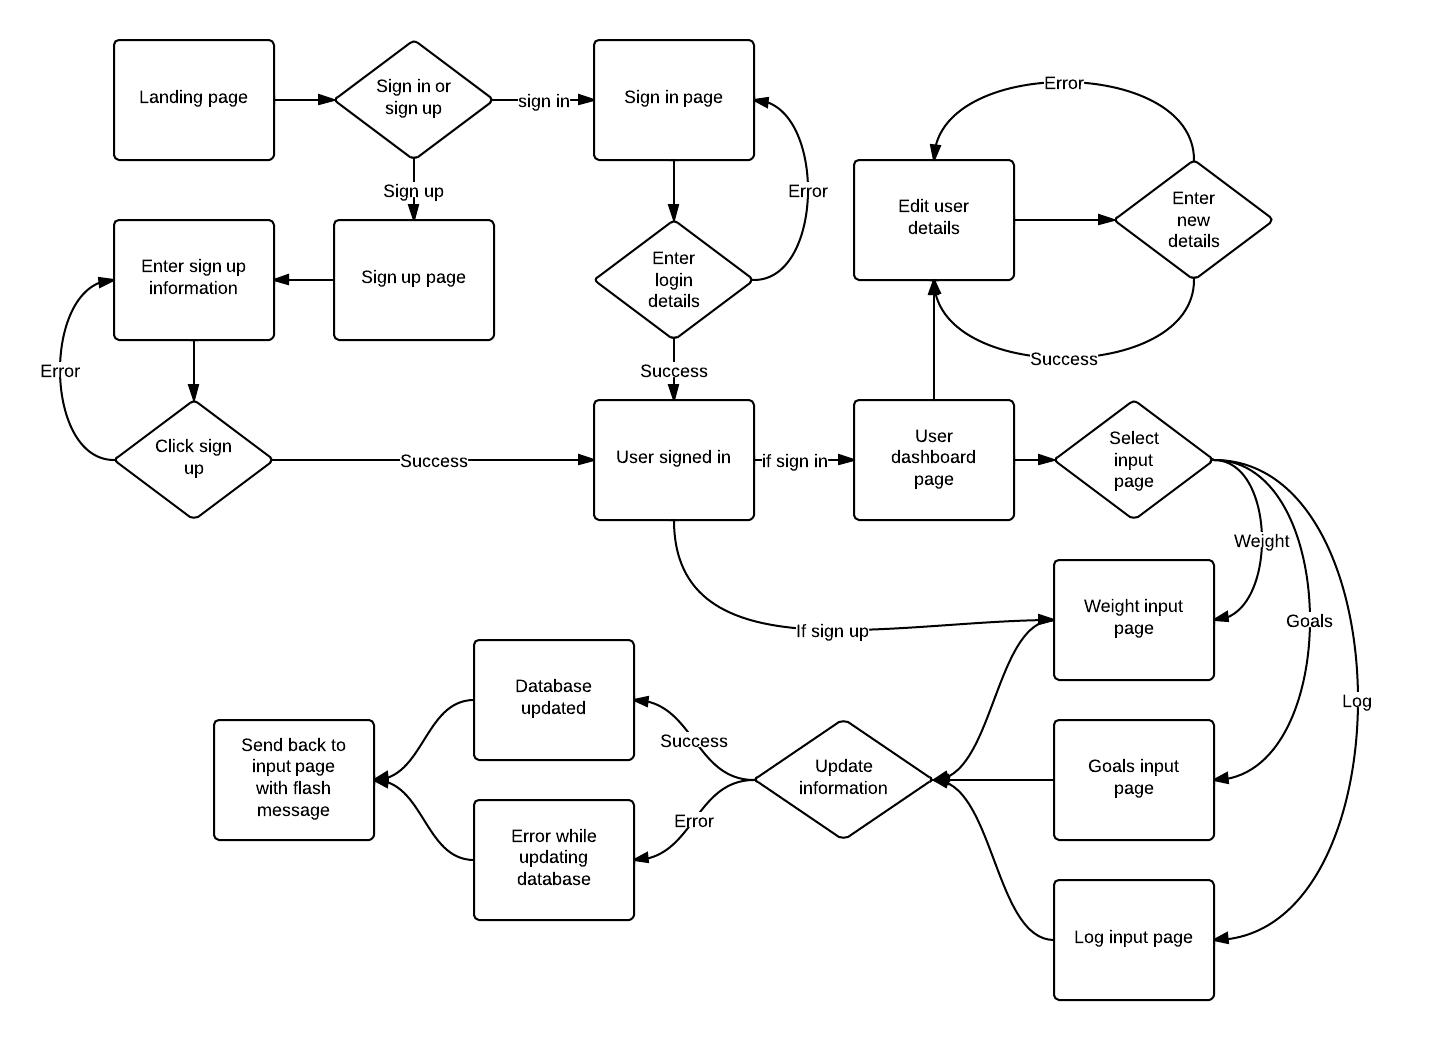
\includegraphics[scale=0.3]{chapters/figs/flowchart}
\caption{Flowchart for the processes and actions of the web application Recur.}
\label{fig:flowchart}
\end{figure}

\section{Design in the browser}
Most of the designs for the application were drawn up, but some of the easier designs were made directly in the browser. This was to speed up the process by cutting out unnecessary tasks. As opposed to the original plan, development begin during the design stage. This was because there was enough of a design to begin developing some of the application. Once development was underway some elements had not been designed yet, for example; the forms for signing in and out. There was a clear vision of what the forms should look like, so instead of wasting time making the wireframe and mock up of them, they were just designed as the web application was being constructed, in the browser. This allows for rapid prototyping of the application's appearance and lessens the work load on the design front, and even if the design does not work there is no reason why another design cannot be drawn up and implemented.\\

\section{Database design}
As well as the design of the application, the design of the backend will need to be done before development takes place. For the backend, Ruby on Rails \citep{rails:2013} will be used. The reasoning behind this will be discussed in the development Chapter \ref{sec:dev} Page \pageref{sec:dev}. A number of attributes will be stored about each user and will be split up over a number of tables. Each table will have a one to many relationship with the user table, apart from the options table with will be one to one. This is because a user will only need to have one set of option in the database at any one time. The other tables will be current are:

\begin{enumerate}
\item Current weight table which will store the current weight of the user.
\item Goal weight table which will store the goal weight of the user.
\item Fitness log table which will store information about what exercises they did and how they did.
\item Goals table which will store the users goals
\end{enumerate}

\noindent
All of these will link back to the user's ID. Originally, there was going to be a user's weight table, which would store both the current and goal weight, but it was moved to two different tables because it is unlikely that the user will be updating the goal weight as much as they were going to update their current weight. All of these tables will depend upon their user, so if the user is removed from the database, their data from the other tables will be removed as well. Below (Figure \ref{fig:erd}) you can see the entity relationship diagram for the application.

\begin{figure}[!ht]
\centering
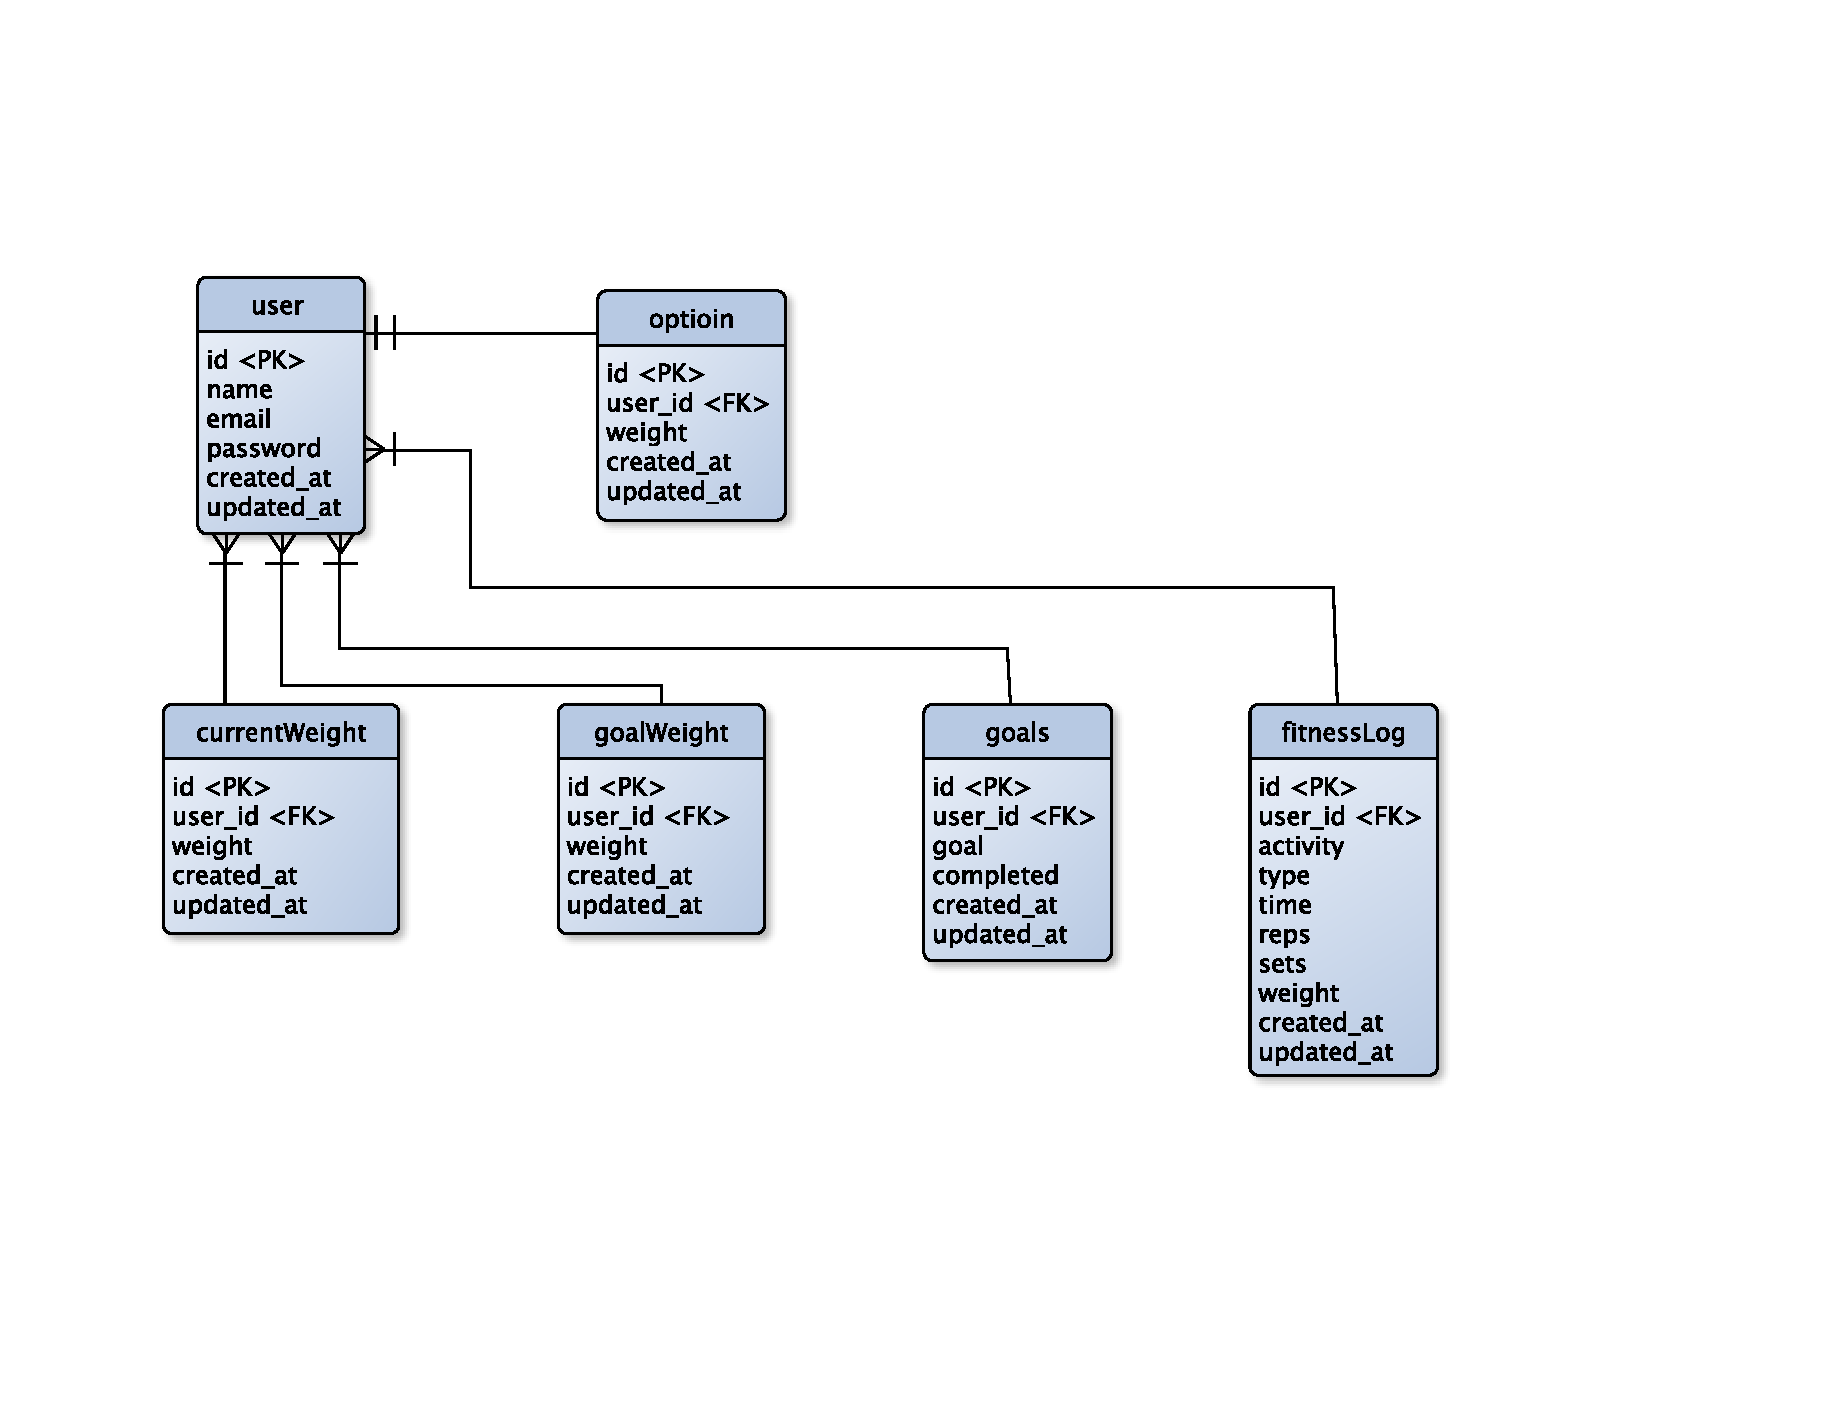
\includegraphics[scale=0.5]{chapters/figs/erd}
\caption{Entity Relationship Diagram for the website application Recur.}
\label{fig:erd}
\end{figure}

\section{Conclusion}
To conclude, designing with the user in mind is priority one. Make sure the application is accessible by almost everyone will give you the widest scope of people that can potentially use your application. Making sure that the application has legible type and a strong contrast between background and font colour is important. Also, with the increase in traffic from mobile devices, designing for the mobile is another major priority. As well as having an efficient design, having an efficient backend is important as well. Making sure the data is stored in a way that will not result in duplicated data and having all of the data easily accessible when needed will result in a smooth running application. All of the information covered at this stage can be handed over and used during development.